\chapter{数学疑难杂症}
\section{直积$\cdot$张量积$\cdot$直和}
物理人在这些概念上往往非常模糊,胡乱使用,现在我们使用物理人的思想来区分下这几个概念。由于这几个概念的使用场景是在量子力学,所以我们在向量空间上讨论这三个运算。

直积和张量积是紧密相连的,这两个概念一起介绍。直积从定义上讲就是给两个集合,然后把两个集合简单的并在一起构成一个更大的集合,$A\times B$,仅此而已。但我们一般会在上面进一步定义内积和加法数乘使得其成为一个线性空间:
\begin{description}
	\item[加法] $(a,b)+(a^\prime,b^\prime)=(a+a^\prime,b+b^\prime)$
	\item[数乘] $\lambda (a,b)=(\lambda a,\lambda b),\quad\lambda\in\mathbb{F}$
	\item[内积] $(a,b)\cdot (a^\prime,b^\prime)= a\cdot a^\prime +b\cdot b^\prime$
\end{description}
这样构成的空间称为$\mathbb{F}$上的自由向量空间:
\begin{equation}
	\mathcal{F}(V,W;\mathbb{F})\equiv \left\{\sum_{(v,w)\in V\times W}k_{v,w}(v,w),k_{v,w}\in\mathbb{F}\right\}
\end{equation}
这个向量空间非常大,就是把每个$(u,v)\in V\times W$都拿来作为基底张成的线性空间。张量积的初衷是想去找$V\times W\to Z$上的双线性函数$f$,双线性函数一定满足下面的条件:
\begin{equation}
	\begin{aligned}&\text{ (}k_1v_1+k_2v_2,w)\sim k_1(v_1,w)+k_2(v_2,w)\\&(v,k_1w_1+k_2w_2)\sim k_1(v,w_1)+k_2(v,w_2)\end{aligned}
\end{equation}
$\sim$表示它们作用$f$得到的值一样。这么来看原先的那个$V\times W$还是太大了,无法自然地蕴含上面的等价关系,所以我们干脆把上面的两条等价关系给模掉,得到一个更合适的线性空间$Y$:
\begin{equation}
	Y\equiv \mathcal{F}(V,W)/\sim
\end{equation}
数学人更喜欢用的不是上面两条,而是和它们等价的下面四条:
\begin{equation}
	\begin{aligned}
		&\begin{aligned}(v_1+v_2,w)\sim(v_1,w)+(v_2,w)\end{aligned} \\
		&\begin{aligned}(v,w_1+w_2)\sim(v,w_1)+(v,w_2)\end{aligned} \\
		&(kv,w)\sim k(v,w) \\
		&(v,kw)\sim k(v,w)
	\end{aligned}
\end{equation}

从$V\times W$到$Y$的线性映射我们记为$h$,则$f$就自然诱导出来了$Y\to Z$的线性映射$g$,而且$Y$也小多了,我们也没必要去强调$g$的双线性性质,现在$Y$自己就蕴含了线性映射的双线性性。我们把这个新的空间叫做$V\otimes W$,即张量积空间。物理上我们把里面的元素写为$\ket{\psi}\ket{\phi}$,而且前面的四条性质就蕴含在我们物理上对张量积的普遍共识,物理上对于张量积的应用一般是体系有多个自由度,比如多个粒子或者一个粒子但是有自旋这种自由度,那么整个希尔伯特空间就看作是每个自由度的希尔伯特空间的张量积。而且在每个自由度上的矢量加法满足$\otimes$的分配律。

由于任何一个映射$f$都可以诱导出映射$g$,所以很多时候我们不会额外区分两者,事实上可以证明双线性映射空间$\mathscr{L}(V,W;Z)$和$\mathscr{L}(V\otimes W;Z)$是同构的。在物理上我们考虑的线性空间都是内积空间\footnote{尽管张量积的定义不需要内积,对偶空间也不需要,这里我们只看有内积的简单情况。},根据里斯表示定理,每个向量空间中的元素都可以和其对偶空间中的元素通过内积双线性性建立一一对应,也即所谓ket和bra的概念。如果取:
\begin{equation}
	(\bra{\psi_1}\otimes\bra{\phi_1})\cdot (\ket{\phi_1}\otimes\ket{\psi_2})=\braket{\phi_1}{\phi_2}\cdot\braket{\psi_1}{\psi_2}
\end{equation}
那么很容易说明$V^*\otimes W^*=(V\otimes W)^*$。当然,这一点的成立并不依赖于上面的内积选取\footnote{毕竟它的定义就不需要内积,这里局限在内积空间上讨论感觉从物理直观上更容易说清楚,用严谨的general的数学反而迷糊。},只是量子力学里面都是这么取的。

上面的定义是构造性的,但数学上更喜欢的是泛性质的定义,直接用下面的交换图就好了:
\begin{definition}
	张量积空间是某个向量空间$Y$ 配以双线性映射 $h:V\times W\to Y$ ,使得对于任意双线性映射 $f:V\times W\to Z$ ,存在唯一的线性映射 $g:Y\to Z$ ,使 $f=g\circ h$ 。
	\begin{center}
		\begin{tikzcd}
			V\times W \arrow[r,"h"] \arrow[dr,"f"]
			& Y= V\otimes W\arrow[d,dashrightarrow,"\exists !g"]\\
			& Z
		\end{tikzcd}
	\end{center}
	上面交换图中虚线的意思是存在且唯一存在一个映射使得图标交换。
\end{definition}

直和和直积在数学上真的不怎么区分,我先给出泛性质的定义你就知道它们之间的区别有多么微妙了。
\begin{definition}
	直积在数学上指的是\textbf{积范畴},即对于范畴 $\mathcal{C}$ 中的一族对象 $X_i\left(i\in I\right)$,若存在一个对象,通常记为 $\prod_{i\in I}X_i$ ,以及一族态射$\pi_j:\prod_{i\in I}X_i\to X_j$使得对任意对象 $X$ 和一族态射$f_j:X\to X_j$,都存在唯一的态射$f:X\to\prod_{i\in I}X_i$使得对任意 $i\in I$ 都有$	\pi_i\circ f=f_i$
	那么对象 $\prod_{i\in I}X_i$ 连同态射族 $\{\pi_i:i\in I\}$ 称为对象族 $\{X_i:i\in I\}$ 的积(product)。画出交换图如下:
	\begin{center}
		\begin{tikzcd}
			X \arrow[r,dashrightarrow,"\exists ! f"] \arrow[dr,"f_j" swap]
			& \prod_{i\in I} X_i\arrow[d,"\pi_j"]\\
			& X_j
		\end{tikzcd}
	\end{center}
\end{definition}

\begin{definition}
	直和在数学上指的是\textbf{余积范畴}(coproduct),交换图上的定义只需要把上面图的箭头全部反转就好了,文字定义不难相应写出:
	\begin{center}
		\begin{tikzcd}
			X \arrow[r,dashleftarrow,"\exists ! f"]\arrow[dr,leftarrow,"f_j",swap]
			& \coprod_{i\in I} X_i\arrow[d,leftarrow,"\iota_j"]\\
			& X_j 
		\end{tikzcd}
	\end{center}
	可见两者定义上差的只是一个是投影$\pi$,一个是嵌入$\iota_i$。
\end{definition}
从范畴的角度看它们差的仅仅只是一个是积一个是余积,把箭头反过来罢了!所以数学上真的不怎么区分,特别是对于线性空间范畴,这个定义真的就是等价的!从维数上也能看出这一点$\mathbb{R}^m\times\mathbb{R}^n=\mathbb{R}^m\oplus\mathbb{R}^n=\mathbb{R}^{m+n}$,但是前面的张量积$\mathbb{R}^{m}\otimes\mathbb{R}^{n}=\mathbb{R}^{mn}$。但是这里说的是外直和,后面还会讲到内直和。

回到物理一些的想法,翻阅喀兴林老师的高量课本,第一章就给出来直和的三条性质:
\begin{description}
	\item[数乘分配]$\lambda \left(\ket{\psi}\oplus\ket{\phi}\right)=\lambda\ket{\psi}\oplus\lambda\ket{\phi}$
	\item[加法] $\ket{\psi}\oplus\ket{\phi}+\ket{\psi^\prime}\oplus\ket{\phi^\prime}=\left(\ket{\psi}+\ket{\psi^\prime}\right)\oplus\left(\ket{\phi}+\ket{\phi^\prime}\right)$
	\item[内积]$\left(\ket{\psi}\oplus\ket{\phi},\ket{\psi^\prime}\oplus\ket{\phi^\prime}\right)=\braket{\psi}{\phi}+\braket{\psi^\prime}{\phi^\prime}$
\end{description}
这不和自由向量空间的定义一模一样么!所以在线性空间范畴上真看不出啥区别。我们再看\textbf{直和}和一般的\textbf{向量的和}有啥区别。注意我们定义主打的就是两个希尔伯特空间是互相分开的,互相不影响,我们在定义两个向量空间的外直和时,我们并不要求两个向量空间的元素之间有加法定义,而是定义直和来把多个自由度强行直接并起来。这其实有某种选择定则在里面,当我们把两个态加起来的时候,我们认为它们处于同一个线性空间,可以叠加得到混合态。但是你绝对不会把一个自旋为0和一个自旋为$\frac12$的态直接叠加起来,因为这意味着一个单粒子态一会儿是费米子,一会儿是玻色子,尽管理论上这种禁闭没有严格证明(见Weinberg场论第一卷相关部分),但是我们从实验上可以相信这种禁闭是存在的,而这个时候考虑总的体系希尔伯特空间,最好的方式就是用直和了,也就是直接直积并起来罢了。

量子力学里面更多的去讲直和是讲巨正则系综构造Fock空间。由于非相对论性的量子力学是个粒子数不变的体系,所以也存在上面与自旋类似的选择定则,也就是说你不会把两个粒子数不同的态直接加起来构造一个混合态,这是没有物理意义的。要用的时候就直接把他们看作是处于完全不同的希尔伯特空间,有自己的一套加法数乘规则,而且互不影响,最后再把它们通过直和直接并起来,构成一个系综,是一个混合态。

内直和就完全不一样了,内直和我们首先是有一个很大的向量空间,然后想去考虑他的分解,但是我们比较关注“正交分解”,也就是说希望把$V$分解为一系列子空间$V_1,V_2,\cdots$,这些子空间互相除了零元素没有公共元素,但它们之间的元素是有子空间自然诱导的加法的。如果对于$V$中的任意一个元素$v$,都存在且唯一一组$(v_1,v_2,\cdots)$使得$v=\sum_i v_i$,则称$V$是$V_1,V_2,\ldots$的(内)直和,也记为:
\begin{equation}
	V=\bigoplus_{i=1} V_i
\end{equation}

在讨论群表示的时候涉及到群表示的分解,那个分解实际上就是在把群表示空间分解为一系列更小的空间的内直和,每个最小的不能再分的块就是不可约表示。在纯粹考虑矩阵理论的时候也会谈及张量积和直和的概念,矩阵的直和应该对应到内直和,而张量积就是前面讨论的张量积(把矩阵看成是线性算符,$V\otimes W$看成是$(V^*\otimes W^*)^*$),只是把前面的理论用线性算符重写了一遍,并选取了一组基底写成矩阵形式。不少文献也把矩阵的张量积叫克罗内克积。

总结一下,这一节定义$V\otimes W$的目的就是把$V\times W$上的双重线性映射提升为新的空间$V\otimes W$上的线性映射来研究。而且$V\otimes W$的本质其实就是$\mathscr{L}(V^*,W^*,F)$,也就是对偶空间上的双重线性泛函,这一点可以从下面的等式看出来:
\begin{equation}
	V\otimes W\cong \mathscr{L}\left((V\otimes W)^*,F\right)\cong\mathscr{L}\left(V^*\otimes W^*,F\right)\cong\mathscr{L}(V^*,W^*,F)
\end{equation}
牢记这一本质,我们可以把$V\otimes W$具体构造出来。首先对于$f\in V^*,g\in W^*$,可以定义这两个线性泛函的张量积为:
\begin{equation}
	(f\otimes g)(v,w)\equiv f(v)\cdot g(w)
\end{equation}
不难发现通过张量积$\otimes$运算,我们从$V,W$中的线性泛函出发得到了一个$V\times W\to F$的双重线性泛函,也就是$V^*\otimes W^*$中的一个元素。同样,假设$V$的基底为$\{e_i|i\in I\}$,$W$的基底为$\{f_j|j\in J\}$,把他们看成是$V^*$和$W^*$中的线性泛函,那么$V\otimes W$的基底就可以构造为:

\begin{equation}
	V\otimes W=\mathrm{span} \left\{e_i\otimes f_j|(i,j)\in I\times J\right\}
\end{equation}
这样我们就找到了$h:V\times W\to V\otimes W$。我们这里都是集中在两个线性空间的基础上讨论,这一构造可以轻易推广到有限个向量空间的张量积上面去,而且不难证明满足结合律,$V\otimes W\otimes Z$是良定义的。

\section{Grassmann几何}
\subsection{外代数}
接着上面一节继续讨论,前面的张量积空间对任意向量空间$V,W$都是可以进行构造的,现在我们把范围搞窄一点,假设只考虑$V$和他的对偶$V^*$构成的张量积空间:
\begin{definition}[$(r,s)$阶张量空间]
	\begin{equation}
	V^r_s=\underbrace{V\otimes\cdots \otimes V}_{r}\otimes \overbrace{V^*\otimes\cdots \otimes V^*}^{s}
\end{equation}
这称为$(r,s)$阶张量空间,其中的$r$叫逆变阶数,$s$叫协变阶数。特别地定义$V^0_0\equiv F$
\end{definition}
\begin{remark}
	实际上这些$V,V^*$完全可以交替排列,不过我们总可以让他们排列成这样整齐的方式便于记号书写方便。
\end{remark}

再来解释一下为什么要叫逆变反变,根据前面说的,我们记$V=\{e_i\},V^*=\{e^{*j}\}$,那么$V^r_s$中的任意一个向量都可以展开为下面的形式:
\begin{equation}
	x=x^{i_1,\ldots,i_r}_{j_1,\ldots j_s}e_{i_1}\otimes\cdots \otimes e_{i_r}\otimes e^{*j_1}\otimes\cdots \otimes e^{*j_s}
\end{equation}
\begin{remark}
	注意一上一下表示求和,不但能帮助我们分清求和指标,还能帮我们分清协变逆变。
\end{remark}

由于$V$中基底$\{e_i\}$的选取是完全任意的,可以差一个线性变换,对应的$\{e^{*j}\}$的选取也就可以差个线性变换,而且是对应的逆矩阵,$x$本身在基底变换下是绝对的,但是其在不同基底下的分量会差个线性变换,可以证明如果选取${A_i}^je_j$作为新基底,$x^i$会利用$A$的逆矩阵变换,所以对应$V$的基底$e_{i}$叫逆变的(尽管本身$e_{i}$用$A$来变);同样的$x_j$会利用$A$矩阵本身来变换,所以对应$V^*$的基底$e^{*j}$叫协变的(尽管本身$e^{*j}$用$A^{-1}$来变)。

$V^r_s$中的元素除了可以用张量积运算生成更大的张量以外,还可以利用缩并这个运算生成更小的张量,数学上严格定义为:
\begin{definition}[缩并]
	张量$x$的缩并定义为:
	\begin{equation}
		\begin{aligned}C_{\lambda\mu}(x)=\langle v_{\lambda},v^{*\mu}\rangle v_{1}\otimes\cdots\otimes\hat{v}_{\lambda}\otimes\cdots\otimes v_{r},\\\otimes v^{*1}\otimes\cdots\otimes\hat{v}^{*\mu}\otimes\cdots\otimes v^{*s},\end{aligned}
	\end{equation}
	其中$\hat{}$表示去掉这个因子。
\end{definition}
不过物理人口中更关心张量的分量,而不是其本身,毕竟分量是用来真正做计算的,那么缩并其实就是把某个上指标和某个下指标去成一样的然后求和,类似于矩阵取trace。

无论是缩并还是张量积,最终得到的元素都不会在原空间里面,这引导我们去利用直和构造Fock空间一样来构造更加大的空间,使得这些运算是封闭的。我们现在只考虑$V^r_0$或$V_s^0$,也就是不考虑$V$和$V^*$的混合:
\begin{definition}[张量代数]
	由所有$T^r(V)\equiv V^r_0(r\geq 0)$的直和构成的空间记为:
	\begin{equation}
		T(V)\equiv \bigoplus_{r=0} V^r_0
	\end{equation}
	显然这个空间没有缩并运算,但是在张量积运算下是封闭的,构成了一个代数,称为\textbf{张量代数}。
\end{definition}

$T^r$空间作为线性空间可以考虑两类子空间,考虑下面两个投影算子:
\begin{equation}
	\begin{gathered}
		S_{r}(x)={\frac{1}{r!}}\sum_{\sigma\in{\mathfrak{ S}_r}}\sigma{x}, \\
		A_{r}(x)={\frac{1}{r!}}\sum_{\sigma\in{\mathfrak{ S}_r}}\operatorname{sgn}\sigma\cdot\sigma x 
	\end{gathered}
\end{equation}
这里$\mathfrak{S}_r$表示$r$阶置换群,上面的两个算子把$T^r(V)$分别投影到全体全对称张量的集合$P^r(V)$和全反对称张量的集合$\Lambda^r(V)$。从指标上看就是那些全对称和全反对称的张量构成的向量空间。显然这个时候如果继续把$P_r(V)$或者$\Lambda^r(V)$直接对所有$r$直和起来的空间在张量积运算下并不构成一个代数,所以要对乘法进行修正,下面具体来考虑反对称部分。
\begin{remark}
	约定$\Lambda^{1}(V)=V,\Lambda^{0}(V)=F$。
\end{remark}
\begin{definition}[外积]
	\begin{equation}
		\xi\wedge\eta=\frac{(k+l)!}{k!l!}A_{k+l}(\xi\otimes\eta),\quad\xi\in\Lambda^k(V),\eta\in\xi\in\Lambda^l(V)
	\end{equation}
	其中$A_{k+l}$是前面定义的反对称化算子。不难验证$\xi\wedge\eta\in\Lambda^{k+l}(V)$。
\end{definition}
外积运算有如下性质:
\begin{itemize}
	\item 分配律:
	\[(\xi_{1}+\xi_{2})\wedge\eta=\xi_{1}\wedge\eta+\xi_{2}\wedge\eta,\quad \xi\wedge(\eta_{1}+\eta_{2})=\xi\wedge\eta_{1}+\xi\wedge\eta_{2}\]
	 \item 反变换律:$\xi\wedge\eta=(-1)^k\eta\wedge\xi$ 
	\item 结合律:($\xi\wedge\eta)\wedge\xi=\xi\wedge(\eta\wedge\zeta)$.
\end{itemize}
\begin{definition}[外代数]
	在上面外积的定义下\[\Lambda(V)\equiv\bigoplus_{r=0}\Lambda^r(V)\]构成一个代数,称为\textbf{外代数},或\textbf{Grassmann代数}。
\end{definition}

\section{李超代数}
物理人群环域模体格这些代数结构真正关心的就是群,而且很多情况下只关心它的表示,为了更好地数学上刻画李超代数,我们从环和域开始讲起。

回忆群的定义,是在集合上定义了一个乘法结构,而且封闭、结合、存在幺元且元素都可逆,现在考虑把这四条性质一条条加上去。如果只有封闭性,则称为\textbf{原群(Magama)},考虑继续加性质:
\begin{definition}[半群与幺半群]
	带有二元运算的非空集 $S$ 若满足结合律,则称之为\textbf{半群}.存在幺元的半群称为\textbf{幺半群(Monoid)}.若$M$ 是幺半群,而子集$M^{\prime}\subset M$ 满足 (i)$M^{\prime\prime}$ 对乘法封闭,(ii) $1\in M^{\prime}$,则称 $M^{\prime}$ 为 $M$ 的子幺半群.
\end{definition}
如果在幺半群的基础上加上所有元素都可逆,那就得到了群的定义。
\begin{definition}
	(含幺)环是一组资料 $(R,+,\cdot)$,其中
	\begin{itemize}
		\item [1.]$(R,+)$ 是交换群,二元运算用加法符号记作 $(a,b)\mapsto a+b$, 加法幺元记为 0, 称之为 $R$ 的加法群;
		\item [2.]乘法运算 $\cdot:R\times R\to R$ 简记为 $a\cdot b=ab$, 满足下述性质:对所有 $a,b,c\in R$, $\diamond a( b+ c) = ab+ ac, \quad ( b+ c) a= ba+ ca\quad ( $分配律,或曰双线性$) , $
		$\diamond\:a(bc)=(ab)c\quad($乘法结合律);
		\item[3.]存在元素 1$\in R$ 使得对所有 $a\in R$ 皆有 $a\cdot1=a=1\cdot a$, 称作 $R$ 的 (乘法) 幺元.
	\end{itemize}
		后面两点其实蕴含了$(R,\cdot)$是一个幺半群。除去和幺元相关性质得到的$(R,+,\cdot)$ 称作无幺环. 若子集 $S\subset R$ 对 $(+,\cdot)$ 也构成环, 并且和 $R$ 共用同样的乘法幺元 1,则称 $S$ 为 $R$ 的子环,或称 $R$ 是 S 的环扩张或扩环.
\end{definition}
\begin{example}
	后面用的比较多的是$\mathbb{Z}_n$环,它的元素由整数关于$n$的模得到,比如$\mathbb{Z}_2=\{\bar 0,\bar 1\}$,加法和乘法就是自然数的加法乘法取模$n$。全体整数也构成一个环,称为自由环$\mathbb{Z}$。
\end{example}
\begin{definition}
	域是一组资料$(K,+,\cdot)$,其中
	\begin{itemize}
		\item [1.]$(R,+)$ 是交换群;
		\item [2.]$(R,\cdot)$ 是交换群;
		\item [3.]$\forall a,b,c\in K,a\cdot (b+c)=a\dot b+a\dot c$.
	\end{itemize}
	这个定义和环颇有些相似,实际上域可以看作是环上的乘法幺半群附加交换性,这时候环变成一个\textbf{交换环},再要求乘法意义上环中除了加法零元每个元素都有逆,这环变成\textbf{除环(体)}。\textbf{域就是一个交换可除环}。
\end{definition}
简单点说就是一个集合上面定义了加减乘除,满足通常的结合律、交换律和分配律等等。但是有一个地方和小学学的数域有点不一样,若干个相同的不为0的数求和可以为0。比如$\mathbb{Z}_2$也可以看作一个域,其中$\bar 1+\bar 1=\bar 0$!
\begin{definition}
	一个域只可能出现两种情况:
	\begin{description}
		\item[特征$0$:] 任何元自己和自己加法无论多少次都不会得到零元(零元自己除外);
		\item[特征$p$:] $\exists p\in\mathbf{Prime}$满足任何数自己和自己相加$p$次后总是得到零元。
 	\end{description}
\end{definition}
后面的讨论在特征为$0$的域上进行。

回忆李代数首先是一个代数,生活在一个线性空间,李超代数首先是一个超代数,和代数的区别是其生活在阶化之后的线性空间上。
\begin{definition}[$Z_n$阶化向量空间]
	若一个向量空间可以直和分解为$V=\bigoplus_{\alpha\in\mathbb{Z}_n}V_\alpha$,则称$V$为$Z_n$阶化向量空间。$V_\alpha$子空间中的元素称为$\alpha$阶齐次元。
\end{definition}
这个定义只要求这样的分解存在就行,并不需要搞清楚$V_\alpha$到底谁是谁。
\begin{theorem}
	若$V,W$都是$Z_n$阶化向量空间则它们上面的线性算子$\mathscr{L}(V,W)$也是一个$Z_n$阶化向量空间。张量积空间亦然。
\end{theorem}
考虑$V$上的双线性函数$f:V\times V\to K$,可以有下面几种形式:
\begin{description}
	\item[相容的:]$\forall x\in V_\alpha,y\in V_\beta,f(X,y)\propto\delta_{\alpha\beta}$
	\item[超对称的:]$\forall x\in V_\alpha,y\in V_\beta,f(X,y)=(-1)^{\alpha\cdot\beta}f(y,x)$
	\item[反超对称的:]$\forall x\in V_\alpha,y\in V_\beta,f(X,y)=-(-1)^{\alpha\cdot\beta}f(y,x)$
\end{description}
\begin{definition}
	超代数是一个$\mathbb{Z}_2$阶化的代数
\end{definition}
原先的李代数的代数乘法只有对易子,现在李超代数的目的就是把反对易子也加进来,而前面先定义阶化的目的就是分清楚哪些元素之间反对易关系,哪些之间是对易关系。
\begin{definition}
	李超代数是一个超代数,且乘法$(\cdot,\cdot)$满足:
	\begin{itemize}
		\item[双线性:] $(\alpha,k_1\beta_1+k_2\beta_2)=k_1(\alpha,\beta_1)+k_2(\alpha,\beta_2)\quad(k_1\alpha_1+k_2\alpha_2,\beta)=k_1(\alpha_1,\beta)+k_2(\alpha_2,\beta)$
		\item[阶化反对易:]$\forall x\in V_\alpha,y\in V_\beta,(x,y)=-(-1)^{\alpha\cdot\beta}(y,x)$
		\item[阶化Jacobi恒等式:]$\forall x\in V_\alpha,y\in V_\beta,\left((x,y),z\right)=\left(x,(y,z)\right)-(-1)^{\alpha\cdot\beta}\left(y,(x,z)\right)$
	\end{itemize}
\end{definition}

超代数是代数直接阶化,但是李超代数并非直接把李代数阶化。和李代数一样,李超代数的李超括号可以直接由超代数的乘法诱导:
$$[x,y]=xy-yx,\quad\{x,y\}=xy+yx$$
超李代数的生成元分为两组$x_i\in\mathfrak{g}_{\bar 0},y_\alpha\in\mathfrak{g}_{\bar 1}$,则对易关系可以写为:
\begin{equation}
	[x_i,x_j]=f^k_{ij}x_k,\quad [x_i,y_\alpha]=F^\beta_{i\alpha}y_\beta,\quad \{y_\alpha,y_\beta\}=A^i_{\beta\alpha}x_i
\end{equation}
且结构常数满足:
\begin{equation}
	f^k_{ij}=-f^k_{ji},\quad F^\beta_{i\alpha}=-F^\beta_{\alpha i},\quad A^i_{\beta\alpha}=A^i_{\alpha\beta}
\end{equation}

实际物理上考虑的是它们的射影表示,所以就跟CFT里面的Virasoro代数一样可以有个中心扩张。虽然Poincar\'e代数的中心扩张总可以消除,但是超Poincar\'e代数在$\mathcal{N}>1$时可以有非平庸的中心荷。李超代数的中心扩张定义和李代数完全一致,只是$c$和其他生成元不是对易,而是超对易,也就是$(c,x)=0,\forall x\in\mathfrak{g}$。

\begin{example}[一般线性李超代数]
	李代数比较重要的是考虑其到$\mathfrak{gl}(n)$的子代数的同态,也就是考虑其线性表示。李超代数这边同样也会考虑表示,这个时候对应的是$\mathfrak{pl}(m,n)$的子代数。考虑任意一个$\mathfrak{gl}(m+n)$中的元素,在某个基底下:
	\begin{equation}
		\begin{pmatrix}A_{m\times m}&B_{m\times n}\\C_{n\times m}&D_{n\times n}\end{pmatrix}=\begin{pmatrix}A_{m\times m}&0\\0&D_{n\times n}\end{pmatrix}+\begin{pmatrix}0&B_{m\times n}\\C_{n\times m}&0\end{pmatrix}
	\end{equation}
	这实际上就已经把$\mathfrak{gl}(m+n)$进行了$\mathbb{Z}_2$阶化,分块对角的是$\mathfrak{pl}(m,n)_{\bar 0}$,斜分块对角的是$\mathfrak{pl}(m,n)_{\bar 1}$。然后在矩阵乘法诱导的$[,]$和$\{\}$下构成李超代数。注意到对于同样一个$\mathfrak{gl}(m+n)$,可以有不同的$\mathbb{Z}_2$阶化方法,所以对于李超代数线性表示空间的维数需要用两个指标$m,n$来标记。
	
	常常对于$\mathfrak{pl}(m,n)$中的元素定义超迹:
	\begin{equation}
		\mathrm{str}\  x\equiv\tr A-\tr D
	\end{equation}
	它与基底选取无关,而且超迹自然诱导出一个$\mathfrak{pl}(m,n)\times\mathfrak{pl}(m,n)\to K$的双线性$\left<x,y\right>\equiv\mathrm{str}\ (xy)$,而且它是相容的,还是不变的,也就是说$\left<(x,y),z\right>=\left<x,(y,z)\right>$。超对易子的超迹必然是0,$\mathrm{str}\ (x,y)=0$。利用超迹还可定义出$\mathfrak{pl}(m,n)$的子代数$\mathfrak{spl}(m,n)\equiv\{x\in\mathfrak{pl}(m,n)|\mathrm{str}\ x=0\}$
\end{example}


李超代数和李代数有许多相似之处,比如同样可以定义单李超代数,可以考虑上面的Killing型和伴随表示,还可以考虑典型代数,用Dykin图和Cartan子代数方法找最高权表示或是对单李超代数进行分类。但是它又有不少不同点需要注意,比如Schur引理不再成立:
\begin{theorem}[超Schur引理]
	设$\rho:\mathfrak{g}\longrightarrow\mathfrak{pl}(V)$是李超代数的一个不可约表示,则与全部 $\rho(\mathfrak{g})$ 可超交换的线性变换,
	$$C(\rho)=\{a\in pl(V)|(a,p(\mathfrak{g}))=0\}$$
	只可能是 $C(\rho)=cI$, 或
	\[C(\rho)=c\begin{pmatrix}I_{n\times n}&b\\b^{-1}&I_{n\times n}\end{pmatrix},\quad c\in K\]
	这种情况要求$n=\dim V_{\bar 0}=\dim V_{\bar 1}$
\end{theorem}
再比如李代数的李定理也不再成立。更多有关李超代数表示论的内容请见\cite{superlie,WLXJ198301002,Kac:1977em}。
\section{切矢,微分,子流形和Frobenius定理}
这些都是微分几何最基础的概念,物理人一般就是凭感觉去定义,这种定义方式一般没问题,我们来看数学人是怎么严格理解这件事情的。为此首先看物理人是如何定义的,引入\href{https://www.damtp.cam.ac.uk/user/tong/gr.html}{David Tong}讲义上面的讲法。
\subsection{切矢和微分}

\section{中心极限定理与随机矩阵模型}\label{B.5}
本节说白了就是在玩$0+0$维的量子场论,为讨论大$N$极限做准备。
\subsection{一些关于概率论的常识}
下文中我们用大写字母表示随机变量,用对应的小写字母表示随机变量的取值,后面讨论的都是连续型随机变量。

设随机变量的PDF(概率密度函数)为$p(x)$,定义其特征函数为傅里叶变换:
\begin{equation}
	\widehat{p}(k)=\langle e^{ikX}\rangle=\int dxe^{ikx}p(x)
\end{equation}
利用它在$k=0$处做形式幂级数可以得到:
\begin{equation}
	\begin{gathered}
		\widehat{p}(k)=1+\sum_{n=1}^{+\infty}\frac1{n!}(ik)^nM_n\\
		M_n=\langle X^n\rangle=\int dxx^np(x)=\left.\left(\frac{\partial}{i\partial k}\right)^n\widehat{p}(k)\right|_{k=0}
	\end{gathered}
\end{equation}
还有一个很有用的概念叫cumulants,或者说叫集团(cluster)n阶矩$K_n$:
\begin{equation}
	\widehat{p}(k)=\exp\left(\sum_{n=1}^{+\infty}\frac1{n!}(ik)^nK_n\right)
\end{equation}
实际计算中需要计算$M_n$,也就是n点关联函数,可以把他表示成集团的和的形式:
\begin{equation}
	\begin{aligned}M_1&=K_1,\\M_2&=K_2+K_1^2,\\M_3&=K_3+3K_1K_2+K_1^3,\\M_4&=K_4+4K_3K_1+3K_2^2+6K_2K_1^2+K_1^4\end{aligned}
\end{equation}
所以求关联函数归结为求cumulants,而且上面的公式也可以用图的形式表示出来。比如$M_3$:
\begin{figure}[H]
	\centering
	\includegraphics{figs/fig1.pdf}
\end{figure}
用圈圈起来的代表一个cluster,里面n个球就代表是$K_n$,最终结果就是把所有的分组方法对应的图加起来,每个图又是集团的乘积。这其实就是在考虑n个不同的球如何用完全一样的盒子进行分类(容量相同的视为完全相同的盒子,不同容量盒子依旧不同)。

现在考虑$N$个独立同分布的随机变量$\{X_i\}$,且设$X=\sum_{i=1}^N X_i$,那么$X$的PDF就可以表达为:
\begin{equation}
	\begin{aligned}
		q(x)&=\int[\prod_idx_i]\delta(x-\sum_ix_i)p(x_1)p(x_2)...p(x_N)\\
		&=\int\frac{dk}{2\pi}e^{-ikx}\int[\prod_idx_i]e^{ik\sum_ix_i}p(x_1)p(x_2)...p(x_N) \\
		&=\int\frac{dk}{2\pi}e^{-ikx}[\int dx'e^{ikx'}p(x')]^N \\
		&=\int\frac{dk}{2\pi}e^{-ikx}\widehat{p}^N(k)
	\end{aligned}
\end{equation}
利用特征的定义,设随机变量的方差为$\sigma$,平均值为$\mu$,则有:
\begin{equation}
	\widehat{p}(k)=\exp\left(ik\mu-\frac12k^2\sigma^2+....\right)
\end{equation}
则最终得到:
\begin{equation}
	q(x)=\int\frac{dk}{2\pi}e^{-ik(x-N\mu)-N\frac12\sigma^2k^2+N\mathcal{O}(k^3)}
\end{equation}
N有限时这个式子很复杂,但是积分换元把$Nk$当整体,不难发现$N\to infty$后上式中的$\mathcal{O}(k^3)$完全可以丢掉得到:
\begin{equation}
	q(x)\to\frac1{\sqrt{2\pi N}\sigma}\operatorname{exp}(-\frac12\frac{(x-N\mu)^2}{N\sigma^2})
\end{equation}
这正是中心极限定理说的事情,这也让我们第一次看到了很多理论在取$N\to\infty$后反倒会变得简单。

\subsection{$0+0$维QFT}
我们的讨论从上一节简化后的大N极限下的情况开始,假设$\mu=0$,这个时候随机变量$\Phi$遵从高斯分布:
\begin{equation}
	P(\phi)=\frac1{\mathcal{Z}}\operatorname{exp}(-\frac12m^2\phi^2)
\end{equation}
这里$\mathcal{Z}$是归一化系数,遵从统计力学的术语,我们叫他配分函数。但是真正能用于计算的配分函数定义是$P(\phi)$的特征:
\begin{equation}
	\begin{aligned}\mathcal{Z}[J]&=\frac{1}{\mathcal{Z}}\int d\phi\exp(-\frac{1}{2}m^2\phi^2+iJ\phi)\\&=\exp(-\frac{1}{2}\frac{J^2}{m^2}).\end{aligned}
\end{equation}
显然$\mathcal{Z}=\mathcal{Z}[J=0]$,这其实就相当于把PDF形变一下,加一个流$J$,我们一般把这个叫\textbf{配分函数}\footnote{或者按照高维QFT的叫法叫\textbf{生成泛函}}。按照前面的讨论,只需要把这个配分函数在$J=0$处做形式幂级数就能得到任意点关联函数,对于高斯情况配分函数可以严格计算出来,所以很简单可以得到:
\begin{equation}
	M_{2n+1}=0,\quad M_{2n}=\frac{(2n)!}{n!2^n}\frac1{m^{2n}}
\end{equation}

真实世界的概率模型不可能是如此简单的高斯分布,但是一般非高斯的我们又不会解,退而求其次,我们考虑一个小扰动:
\begin{equation}
	P(\phi)=\frac1{\mathcal{Z}[g]}\exp(-\frac12m^2\phi^2-\frac1{4!}g\phi^4),\quad g\ll 1
\end{equation}

即使是如此简单的扰动就算是计算归一化系数都很困难。注定只能做微扰展开求解,也就是把最终答案写成关于$g$的幂级数。这其实涉及到收敛半径这一比较微妙的问题,高维QFT比如QED,QCD这些模型,展开半径都是0!微扰展开实际上只能理解为渐近展开!但是我们考虑的$0+0$维QFT其实就是微扰方法算一元函数积分,我们不需要care所谓非微扰效应,圈图发散,重整化这些玩意儿。但是这个玩具模型能很好地帮助理解费曼图是怎么来的。

考虑生成泛函:
\begin{equation}
	\mathcal{Z}[g,J]=\frac1{\mathcal{Z}[g]}\int d\phi\exp(-\frac12m^2\phi^2-\frac1{4!}g\phi^4+iJ\phi)
\end{equation}
显然$\mathcal{Z}[g,J=0]=1$,如果微扰地计算出了这个函数。那么直接根据$M_n=\left(\frac{\partial}{i\partial J}\right)^n\mathcal{Z}[g,J=0]$就可以得到任意阶关联函数的微扰解。我们记未受到扰动的Gauss型随机变量的配分函数为$\mathcal{Z}_0[J]$:
\begin{equation}
	\mathcal{Z}_0[J]\equiv \int d\phi \exp(-\frac{1}{2}m^2\phi^2+iJ\phi)
\end{equation}
\begin{remark}
	注意这里定义丢掉了归一化因子$\mathcal{Z}$。
\end{remark}
则:
\begin{equation}
	\mathcal{Z}[g,J]=\frac{1}{\mathcal{Z}[g]}\exp\left[-\frac1{4!}g\left(\frac{\partial}{i\partial J}\right)^4\right]\mathcal{Z}_0[J]
\end{equation}
虽然$\mathcal{Z}_0[J]$可以严格求解,但是我们还是写下他的级数形式,将上面的配分函数写为:
\begin{equation}
	\mathcal{Z}[g,J]=\frac1{Z[g]}\sum_{V=0}^{\infty}\frac{1}{V!}\left[\frac{1}{4!}{-g}\left(\frac{\partial}{\partial J}\right)^4\right]^V\times \sum_{P=0}^{\infty}\frac{1}{P!}\left[\frac12 (-J)\frac{-1}{m^2}(-J)\right]
\end{equation}
我们对因子的$-1$相位进行了合理排布,没那么神秘,只是为了后面计算稍微方便一些,正统QFT,这些相位不是以$-1$给出,而是以$i$的形式给出。费曼图也没那么神秘,无非就是现在想算这个配分函数,每次都一项项展开分析太麻烦了,然后就想了个办法把这些求和中的项用图的形式写出来而已。\footnote{严格来说是费曼图的毛胚版本,正统的费曼图要cut掉外源得到关联函数,然后用LSZ公式使外线在壳,最后发现动量守恒只有那些连通图有贡献,那些图再用波浪线表示光子,实线表示费米子等等美化记号,就得到了通常我们看到的费曼图。}

首先看下求和里面有些啥,首先有$J$,而且很容易求出剩下$E=2P-4V$个,这也直接给出限制$E\geq 0$。其次有$\frac{-1}{m^2}$和$-g$,而且一个$-g$的出现总是意味着四个$-1/m^2$,还有一个归一化因子$\mathcal{Z}[g]$,我们先不管它。这样我们就得到了三个拼图:
\begin{figure}[H]
	\centering
	\includegraphics{figs/fig2.pdf}
	\caption{费曼图拼图}
\end{figure}

唯一要做的事情就是把这些拼图拼起来得到一个闭合的图,所谓闭合,我的意思是说顶点和源或者源和源之间都用传播子粘好了,不存在还剩下半截传播子露在外面的情况,图是连通的还是非连通的倒无所谓。首先从符号上我们知道应该有$(-1)^{P-V}$因子,用这些拼图拼好的闭合的图正好有这样的因子。还有一个问题是为啥引入微扰的时候系数要加个$1/4!$,这也不神秘,首先注意到$V$个顶点$P$个传播子的项数理论上来说由$\partial/\partial J$湮灭$J$的方式决定,总共有$(2P)!/(2P-4V)!$种不同的湮灭方式,不过这里绝大部分所对应的图的拓扑结构都是一样的,也就会对应一样的代数项,当然也有拓扑结构不一样的,所以微扰展开里面的每一项都要用几个拓扑结构不同的图来表示,也就是那些所有具有$P$个传播子,$V$个顶点的图。那些拓扑结构相同的图我们当然只用画一次,然后在前面乘上个系数就好,但是我们并不希望这个系数特别大,即使是泰勒展开前面就有的系数也不能完全把他们消除为1,所以我们预先在$\phi^4$前面乘上了一个$1/4!$。但是事与愿违,这还是不能保证每个图前面的系数都为$1$,但是幸运的是,这个系数只和图的拓扑结构有关,有系统的方法数出来,只是数起来非常麻烦罢了。我这里不打算讲怎么数这些不同的\textbf{对称因子},\href{https://person.zju.edu.cn/yuan}{袁野老师的讲义}上写的很清楚,关于$\phi^4$理论,文献\cite{Palmer:2001vq}中还给出了公式。

继续发挥注意力,注意到求关联函数的时候要对配分函数关于$J$求导,所以$n$点函数肯定不会有$E<n$的贡献,而且最后还要取$J=0$,$E>n$的贡献也没有,所以我们只需要画出那些$E=n$的图。图是正必须$g^V$的,所以从微扰论角度看我们只需要画出少顶点的图。但即使是这样图原则上来说也有无限多,我们画出$V\leq 2$的前面几个,对称因子已经写出来了:
\begin{figure}[H]
	\centering
	\includegraphics{figs/fig3.pdf}
	\caption{$\left<{\Phi^4}\right>$直到$g*2$阶}
\end{figure}
就算这样也有无穷多项,罪魁祸首是那些不带源的图,它们总是有无穷多项,可以和带源的图结合起来得到一个非连通图,而且不增加$E$。但是注意到上面的这些图可以因式分解为下面两个部分:
\begin{figure}[H]
	\centering
	\includegraphics{figs/fig4.pdf}
	\caption{不含真空图的费曼图}
\end{figure}
\begin{figure}[H]
	\centering
	\includegraphics{figs/fig5.pdf}
	\caption{真空图求和}
\end{figure}
设想我们对$\mathcal{Z}[g,J]$已经微扰地画出了所有图,我们把$J$取成0,那些带源地图全部都会变成零,剩下的就只剩下真空图求和了!所以归一化系数$Z[g]$其实就是真空图的求和!注意,我们所有的到现在的讨论都有一个前提,我们忽略了$\mathcal{Z}[g,J]$前面带的$\mathcal{Z}[g]$,结合起来真空图就被自然消除了!其实这是非常自然的,因为归一化系数总是可以吸收进积分测度里面,所以我们甚至可以直接把那些真空图求和归一化为1,不少QFT教材就是直接这么做的,这里是为了让你更直观的看到这些真空图求和怎么被消去的。所以我们只需要考虑那些不带真空图的图,这使得计算得到了大幅简化,不难计算得到(别忘了最后要对$iJ$偏导,这相当于砍掉外源但是保留相连的传播子,仍然离壳):\footnote{注意到我们还能画出一些只有一个源的图的求和,这些图我们称为tadpole,它们求和会对$\left<\Phi\right>$的计算有贡献,在$\Phi^4$理论中由于积分的对称性可以直接看到它们必然为0,但是$\Phi^3$就会出问题,这在我们这里考虑的微积分问题倒没太大问题,但量子场论散射的LSZ框架下必须要求$\bra{0}\Phi\ket{0}=0$!所以我们需要在原先的拉氏量中引入$Y\Phi$重整化项来消除tadpole。}
\begin{equation}
	\langle\Phi^4\rangle=3\frac1{m^4}-4g\frac1{m^8}+\frac{33}4g^2\frac1{m^{12}}
\end{equation}
计算$M_n$我们依旧要画很多图,我们来看下$K_n$的计算会有哪些不一样,$M_n$都可以用$K_n$集团展开表示出来,按理说应该会简单一些。如果一个非连通图可以拆分成几个连通分支,有$n$个不同拓扑结构的连通分支,且每个拓扑构型有$m_i$个子图,那么就会对对称因子有贡献$\frac1{m_1!\cdots m_n!}$,这一简单的排列组合的想法可以帮助我们把所有费曼图的求和(已经把真空图去掉了)化为一堆连通图的求和(对应的对称因子不变,依旧看拓扑结构),不难证明\footnote{这个是真的不难,画一画就好了,详细说明可以见Kerson Huang统计力学的集团展开部分}:
\begin{equation}
	\mathcal{Z}(g,J)=\mathrm{e}^{W_c[J]}
\end{equation}
这里$W_c$意思是所有除去真空图的连通费曼图的求和(带对称因子),显然$W_c[J=0]=0$。把它关于$iJ$展开:
\begin{equation}
	W_c[J]=\sum_{n=1}^\infty \frac{1}{n!}(iJ)^n \left(\frac{\partial }{i\partial J}\right)^n W_c[J=0]
\end{equation}
根据$W_c[J]$的定义,他是我们计算$M_n$的时候的费曼图的那些连通图构成的集合,那显然$\left(\frac{\partial }{i\partial J}\right)^n W_c[J=0]$的意义就是计算$M_n$的时候的连通费曼图的贡献!这一下子要画的图就少了许多,不难看出最后得到的结果就是$K_n$!也就是说$K_n$实际上是$M_n$中那些连通图的贡献,所以很多时候我们也记$K_n=\left<\Phi^n\right>_C$。比如对于$K_4$:
\begin{equation}
	K_4=-g\frac1{m^8}+\frac72g^2\frac1{m^{12}}
\end{equation}
计算的时候最烦人的应该就是图前面的对称因子了,但是可以证明,在计算$K_n$时,也就是计算连通图贡献时,虽然每个图前面都有对称因子,但是由于最终结果是要对$iJ$求偏导得到的,也就是砍去外腿不同的方式又会贡献一个因子,可以和图前面的对称因子相抵消,而且树图这种抵消是精确的!这在上面$K_4$的表达式上也有体现。
\begin{remark}
	你可能会觉得$M_n$才是真正要关心的,$K_n$算出来了只是原则上可以组合得到$M_n$。事实上在量子场论中,由于最终的可观测量不是关联函数本身,而是加上LSZ公式后得到的散射振幅,而LSZ公式干的第一件事情就是让外腿在壳(回忆用$\partial/\partial J$只是砍掉了外源没有扔掉传播子),第二步就是因为每个顶角动量守恒,所以真正有贡献的只有那些连通图!也就是说对散射振幅有贡献的是$\left<\Phi^n\right>_C\subset\left<\Phi^n\right>$,前者只需要画出连通图求得$K_n$再对$iJ$求导,后者需要求出$K_n$,然后放到$e$指数上面,然后再对$iJ$求导,等价于对所有图(连通或者非连通)求和后求导。
\end{remark}

这里我们只考虑了实的随机变量,实际上也可以考虑复随机变量,仍旧可以绘制费曼图求解,但是由于概率必须是实数,所以对图的绘制做了一些要求,这其实类似于费米子费曼图的绘制,或者说复标量场的费曼图绘制,这部分核心思想就是前面那些,只是为了满足一些特定的配对规则多引入了一些规矩而已,也没必要再花时间讲了。

\subsection{所以什么是正统的费曼图?}
	这里考虑的是最简单的$0+0$的QFT,如果随机变量随时间演化,从概率模型变成了随机过程,那么考虑的就是$0+1$维QFT,就是量子力学!那些$\Phi$就可以解释为波函数。
	
	进一步如果$\Phi$还和空间位置有关,成为了一个场,那么我们就得到了$d+1$维QFT,在正则量子化框架下是把这些场看作算符然后加上对易关系,这一做法是必要的,能更好解释粒子态,散射理论这些。不过我们一旦知道我们要计算的其实就是关联函数之后,就好说了,从路径积分的语言来看,要算的关联函数其实就是$n$阶矩,而路径积分算的就是配分函数。只是积分测度从$d\phi$变成了无穷维的$\mathcal{D} \phi$,被积函数$e$指数上面的东东变成了$e^{iS}$,$S$是作用量,对于自由场就是高斯函数的积分。从配分函数得到关联函数同样是求导,只是这个时候求的是泛函导数。总之区别不大,但是费曼图里面的顶点,传播子这些都不是一个单纯的数了,而是一个对空间的积分,而这将意味着圈图带来发散,所以需要做重整化抵消这个发散。然后出来一个Wilson去解释大家这么胡乱地做,去抵消发散到底是有啥物理上的考量,给了个很好地物理图像,然后我们就可以安心地去用Wilson之前大家就发明地维数正规化,PV正规化等等去处理发散问题了。
	
	当然,就像前面说的,我们画的费曼图和经常看到的很不一样,因为我们是带着源的,实际最终还要cut掉源然后代入LSZ公式求散射振幅,这个过程实际上可以打包处理,只要我们升级一下前面画的费曼图,把所有外源提前cut掉,然后LSZ公式外线在壳。再引入一些费曼规则,这样就得到了位置空间的费曼图,顶点传播子这些都是要对空间积分的,但是这依旧很麻烦,毕竟要做积分。事实上我们可以做个傅里叶变换,在动量空间看这些玩意儿,每个顶点的动量守恒自然就从对空间的积分给出来了,而且会消掉很多东西,最后把总体外线的动量守恒$i\delta\left(\sum_i p_i\right)$抽出来,就直接得到了动量空间的费曼规则,把每个线用一些特定的符号画的美观一点,就成了一般大家口中的费曼图。
	
	\begin{figure}[H]
		\centering
		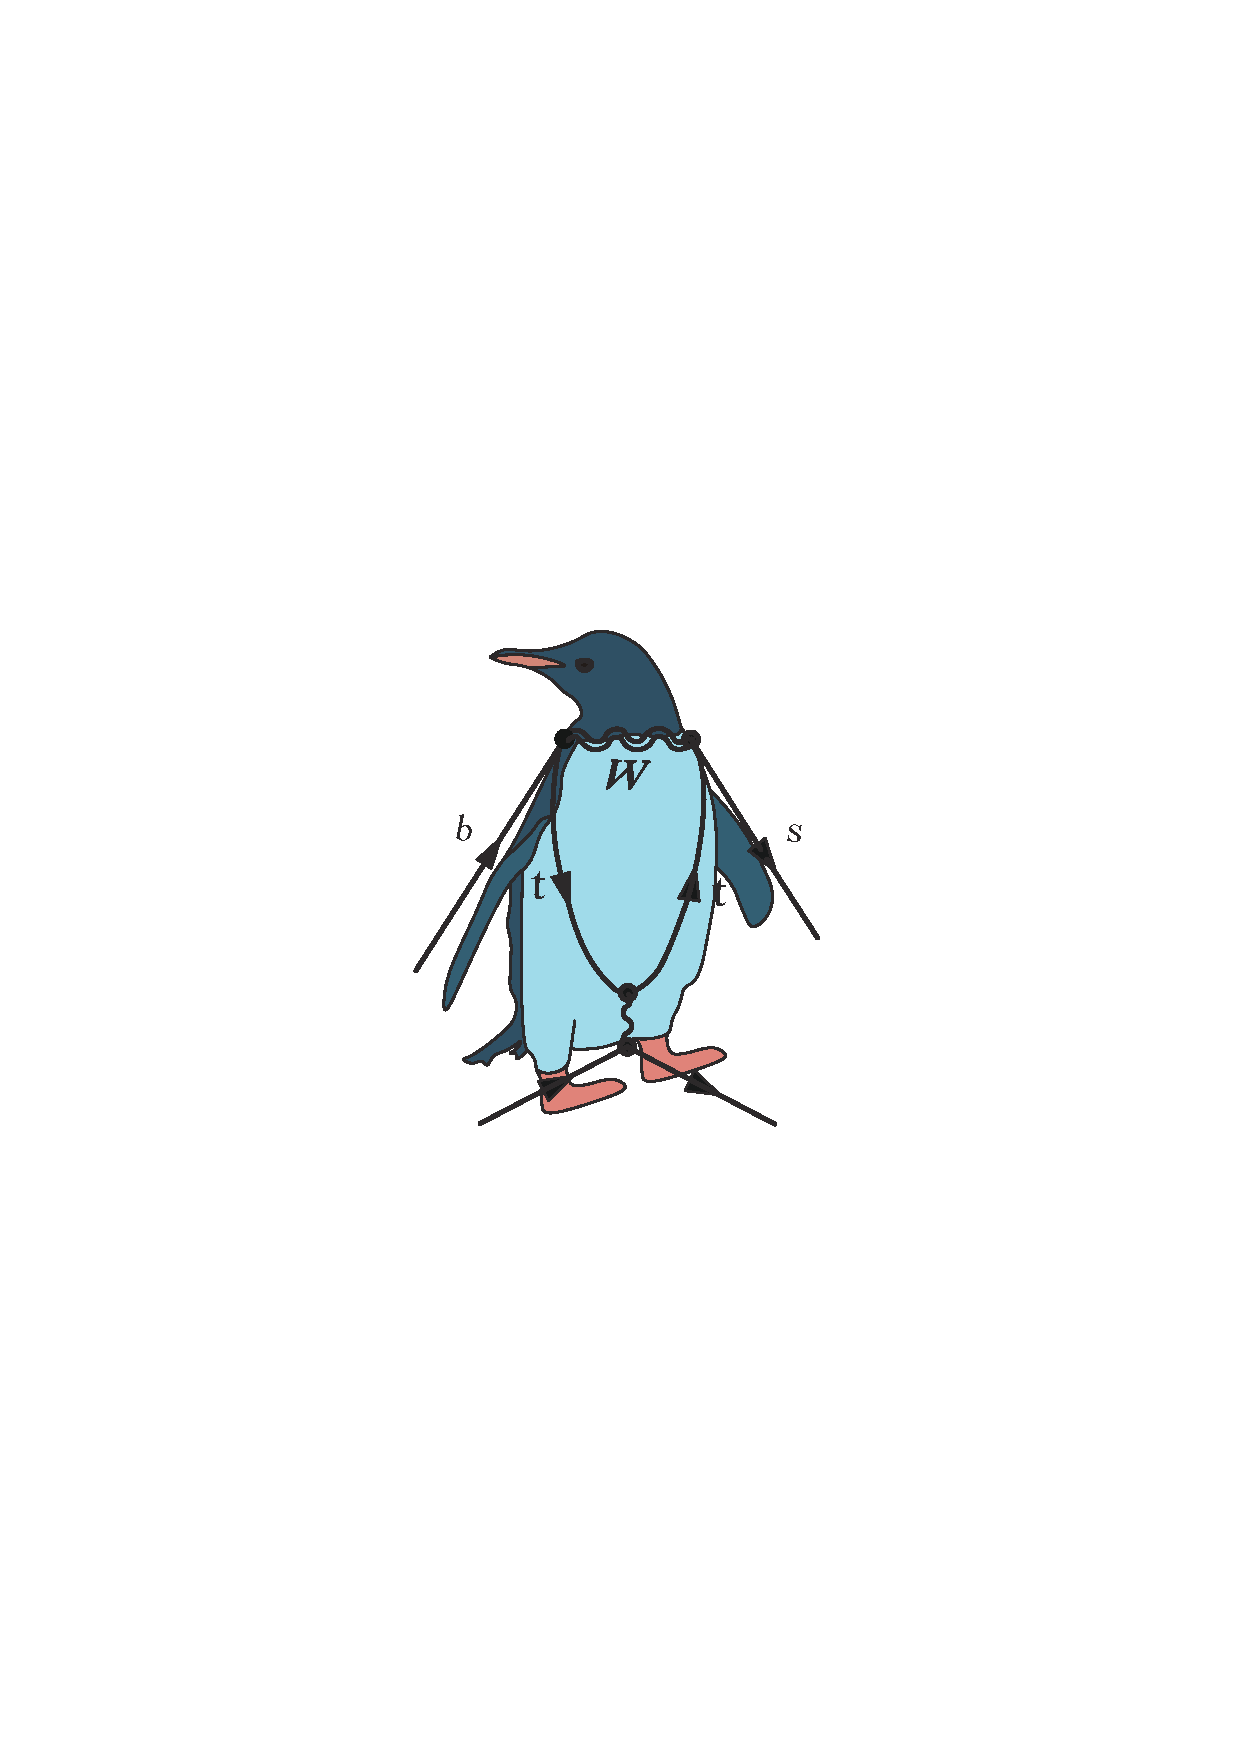
\includegraphics[scale=0.3]{figs/penguin.pdf}
		\caption{老百姓口中的费曼图}
	\end{figure}
	
	常用的那些模型大家都帮你把费曼规则给弄出来了。但是这些费曼规则会非常复杂,要求和的图也非常多,所以现代微扰量子场论(pQFT)重要分支——散射振幅的目标就是脱离费曼图,直接从拉氏量出发,甚至从理论的一些基本假设出发bootsrap出散射振幅。
\subsection{随机矩阵模型}
再来看一个$0+0$维量子场论的例子,随机矩阵模型,他的大N极限形式和QCD的非常相似。

随机矩阵模型就是把一堆矩阵作为系综,比如我们下面考虑$N\times N$的厄米矩阵,矩阵作为随机变量的概率分布为:
\begin{equation}
	P(\phi)=\frac1{\mathcal{Z}}\exp{(-N\text{Tr}V(\phi))}
\end{equation}
假设现在不断地从矩阵空间中选取一个矩阵,选完之后记录下它的特征值,随着选取的矩阵数目越来越多,画出的特征值分布的柱状图越来越趋近于一个光滑曲线$\rho_N(E)$,显然这个PDF可以严格定义为:
\begin{equation}
	\rho_N(E)=\frac1N\langle\text{Tr}\delta(E-\Phi)\rangle=\frac1N\langle\sum_i\delta(E-E_i)\rangle 
\end{equation}
下面我们就是要研究随着$N\to\infty$,$\rho_N(E)$将趋近于怎样的一个函数。定义:
\begin{equation}
	G(z)=\frac1N\left\langle\text{Tr}\frac1{z-\Phi} \right\rangle
\end{equation}
然后利用数学公式:
\begin{equation}
	\operatorname*{lim}_{\epsilon\to0}\operatorname{Im}(\frac{1}{x+i\epsilon})=-\pi\delta(x)
\end{equation}
得到:
\begin{equation}
	\rho(E)=-\frac 1\pi\lim_{\epsilon\to0}\operatorname{Im}G(E+i\epsilon)
\end{equation}
为了进一步简化计算,我们先来看一下矩阵空间的测度$[d\phi]$。可观测量$\Tr\left(\mathcal{O}(\phi)\right)$利用概率分布计算式为:
\begin{equation}
	\langle\mathrm{Tr}(\mathcal{O}(\phi))\rangle=\frac1{\mathcal{Z}}\int[d\phi]\mathrm{Tr}(\mathcal{O}(\phi))e^{-N\mathrm{Tr}V(\phi)}
\end{equation}
可以把测度自然的定义为$[d\phi]\equiv\prod_{p,q}d\phi^p_q$,这个测度在幺正变换下是不变的,而且幺正变换下$P(\phi)$和$\Tr\left(\mathcal{O}(\phi)\right)$都不变,所以整个理论是具有$SU(N)$对称性的。我们改写一下测度使其更明显一些,考虑把测度中的每个$\phi$用某个幺正矩阵$U$对角化为$\Lambda=\mathrm{diag}(\lambda_1,\ldots,\lambda_N)$,则测度一定可以重写为:\footnote{这一节我把它放在了数学附录,但实际上处理的方法优势物理学家所习惯的,但讨论的确确实实又只是数学问题。}
\begin{equation}
	\langle\mathrm{Tr}(\mathcal{O}(\phi))\rangle=\frac1{\mathcal{Z}}\int_{SU(N)}[dU]\int J\prod_id\lambda_i\sum_j(\mathcal{O}(\lambda_j))e^{-N\sum_kV(\lambda_k)}
\end{equation}
这里$[dU]$是$SU(N)$上的Haar测度,而$J$是变换的雅可比行列式。从这个式子可以看出来$[dU]$是可以单独积出来的,结果是$SU(N)$流形的体积,我们完全可以把他归一化为1,得到:\footnote{实际计算当然是前面对测度自然的定义更舒服}
\begin{equation}\label{B.47}
	\langle\mathrm{Tr}(\mathcal{O}(\phi))\rangle=\frac1{\mathcal{Z}}\int J\prod_id\lambda_i\sum_j(\mathcal{O}(\lambda_j))e^{-N\sum_kV(\lambda_k)}
\end{equation}

现在理论的自由度从原先的$N^2$个减少到了$N$个,也就是说我们只需要关心矩阵的本征值!而不是矩阵本身,我们把矩阵的PDF变成了所有矩阵的谱的PDF!这也是很好理解的,因为矩阵模型一直在强调取trace,而且我们还明白了$SU(N)$对称性是这个理论的数学描述上的冗余!这也是为什么前面说矩阵模型和QCD非常像,实际上QCD完全可以用矩阵的形式去写,不像QCD一样需要引入FP鬼场去消除冗余,矩阵模型的冗余非常容易因子话出来并扔掉。实际上这里还剩下个雅可比行列式,这玩意儿其实就是QCD里面鬼场出来的项,也可以用加鬼的方法来物理地求出这个$J$,这里直接给出结果:
\begin{equation}
	\begin{aligned}J=\prod_{i<j}(\lambda_i-\lambda_j)^2\end{aligned}
\end{equation}
我们后面再回过头继续看这个,我们现在先局限于$V(\phi)=-\frac12m^2\phi^2$,也就是先考虑最简单的高斯型,上面的分析告诉我们幺正变换不会改变矩阵元的关联函数:
\begin{equation}
	\left<U^\dagger \phi U\right>=\left<\phi\right>
\end{equation}
利用这一点可得:
\begin{equation}
\begin{aligned}
		G^i_j(z)&\equiv\left<\left(\frac1{z-\Phi}\right)^i_j\right>=\left<\left(U^\dagger\frac{\delta}{z-\lambda_i} U\right)^i_j\right>=\left<\left(\frac{\delta^i_j}{z-\lambda_i}\right)\right>\\
	&=\frac1N\left\langle\text{Tr}\frac1{z-\Phi} \right\rangle\delta^i_j=\delta^i_j G(z)
\end{aligned}
\end{equation}
这里倒数第二个等号利用了在平均的意义下矩阵的$\lambda_N$都是相等的,所以都等于trace的均值再除掉$N$去做平均。现在计算$\rho(E)$约化为计算$G^{i}_j(z)$,而这一函数可以利用泰勒展开写成:
\begin{equation}
	G_j^i(z)=\sum_{n=0}^\infty\frac{1}{z^{2n+1}}\langle\left(\Phi^{2n}\right)_j^i\rangle=\delta_j^i\frac{1}{z}+\frac{1}{z^3}\langle\left(\Phi^2\right)_j^i\rangle+\frac{1}{z^5}\langle\left(\Phi^4\right)_j^i\rangle+....
\end{equation}
说白了就是要求关联函数,然后你可能想着去给PDF加源得到配分函数,然后用前面展开的方法得到费曼规则。但是实际上矩阵模型的费曼规则这样做很复杂,带源的矩阵模型可以参见\cite{Brezin:2016eax},矩阵模型的费曼规则其实是直接“看”出来的。我们首先看两点关联函数:
\begin{equation}
	\langle\Phi_j^i\Phi_l^k\rangle=\frac1{\mathcal{Z}}\int[d\phi]\phi_j^i\phi_l^k\exp\left(-N\frac12m^2\sum_{p,q}\phi_q^p\phi_p^q\right)=\delta_l^i\delta_j^k\frac1{Nm^2}
\end{equation}
由于Gauss型矩阵模型类似于自由场,有类似的Wick定理,可以把多点关联函数转换为两点关联函数之间的组合\footnote{笑,前面几节都在用路径积分的方法算东西,现在回到正则量子化的数学工具反而更舒服。}
\begin{theorem}[矩阵模型的Wick定理]
	\begin{equation}
		\left<\Phi^i_j\cdots\right>=\text{所有可能的缩并}
	\end{equation}
	比如:
	\begin{equation}
		\begin{aligned}
			\left<\Phi^i_j\Phi^k_l\Phi^m_n\Phi^h_t\right>=\wick{\c\Phi^i_j\c\Phi^k_l}\wick{\c\Phi^m_n\c\Phi^h_t}+\wick{\c1\Phi^i_j\c2\Phi^k_l\c1\Phi^m_n\c2\Phi^h_t}+\wick{\c2\Phi^i_j\c1\Phi^k_l\c1\Phi^m_n\c2\Phi^h_t}
		\end{aligned}
	\end{equation}
	这里$\wick{\c\Phi\c\Phi}$的意思是$\left<\Phi\Phi\right>$。这也暗示了所有的$n$为奇数的关联函数都得到0,这从积分的对称性也能看出来。
\end{theorem}
这个定理证明起来并不复杂,看些$N$比较小的例子就能相信他的正确性了。我们再来看一下$G^i_j$的展开式里面有什么,首先注意到每项都可以提出来一个$\delta^i_j$,其次是$1/z$可以理解为传播子,然后是$\Phi$的关联函数,利用前面的Wick定理得知其可以看作是一堆两两配对的组合,为了更好地体现具体是哪两个$\Phi$场配对,我们可以引入所谓double line记号:
\begin{figure}[H]
	\centering
	\includegraphics{figs/fig6.pdf}
	\caption{矩阵模型的费曼图}
\end{figure}
上图中第一个是标记两个矩阵配对的,带来一个传播子,在QCD里面这实际上对应胶子传播子,而且注意到两个箭头相反,都是下指标指向上指标。第二个在QCD里面可以理解为夸克传播子\footnote{这一个指标在图上我们没有画出来,也就是说原则上你可以让第二幅图作用分别带指标$i,j$,然后传播子变为$1/z\delta^i_j$,实际上所有的QFT里面的费曼图都可以这么做,把指标完全写出来,只是由于目前没有哪个理论会让某个粒子传播之后自动变成另一个“味”的粒子,所以都会有个$\delta^i_j$。},毕竟规范场才是带两个指标的矩阵场(因为和生成元结合),夸克场都只带一个指标。实操一下你就懂了。
\begin{example}
	比如$\frac1{z^3}\left<\Phi^i_k\Phi^k_j\right>$可以用下面的图表示为:
	\begin{figure}[H]
		\centering
		\includegraphics{figs/fig7.pdf}
	\end{figure}
	这里一个圈代表指标取相同进行求和缩并,所以这里$k=l$。由于要进行求和,所以理论里面的一个圈就会带来一个$N$,注意,这里说的圈是选取某个单线,沿着箭头走,能回到原点的单线个数。然后由于两边各有一个单外线,所以给一个因子$\delta^i_j$,再看双线有一条,所以给一个双线传播子$\frac1{Nm^2}$,最后再看水平方向有几根单线,这里显然有三段单线,所以给传播子$1/z^3$。最终结果为$\delta^i_j/m^2$。
	
	再看一个复杂点的例子$\frac1 z^5\left<\Phi^4\right>$,首先先画四根柱子:
	\begin{figure}[H]
		\centering
		\includegraphics{figs/fig8.pdf}
	\end{figure}
	然后再考虑怎么连柱子,也就相当于在考虑如何用Wick定理,找不同的缩并方式,事实证明有下面三种:
	\begin{figure}[H]
		\centering
		\includegraphics{figs/fig9.pdf}
	\end{figure}
	把这三种加起来就得到总的值,注意,(a)和(c)两个图是平面图,它们给出的项是高于$\mathcal{O}(1/N)$的,因为含有额外的圈,而(b)这种画在平面上一定有交叉的图,圈为0,给出的项会在$N\to\infty$时被压低!这是大N极限理论的普遍性质,只需要考虑那些平面图!
\end{example}
\begin{theorem}[魏格纳半圆定律]
	在$N\to\infty$时,Gauss型随机矩阵模型本征值PDF有如下简单的形式:
	\begin{equation}
		\rho(E)=\frac{m^2}{2\pi}\sqrt{\frac4{m^2}-E^2},\quad E\in[-2/m,+2/m]
	\end{equation}
\end{theorem}
\begin{proof}
	考虑一个典型的图:
	\begin{figure}[H]
		\centering
		\includegraphics{figs/fig10.pdf}
	\end{figure}
	显然它可以分解为两个更小的图,中间用一个$1/z$传播子连起来,这些最小的不能再分的图,也就是所谓的单粒子不可约图都是用嵌套一个双线或者重复相连多个图得到的。所谓单粒子不可约,就是不能通过剪短一个传播子使得图变成非连通图。略去$\delta^i_j$,$G(z)$就是所有图的叠加,可以用单粒子不可约图的求和表示为:
	\begin{equation}
			G(z)=\quad\frac1z+\frac1z\Sigma(z)\frac1z+\frac1z\Sigma(z)\frac1z\Sigma(z)\frac1z+...
			=\frac1{z-S(z)}
	\end{equation}
	反过来,在$G(z)$上面嵌套一个双线又得到所有的单粒子不可约图求和:
	\begin{equation}
		S(z)=\frac1{m^2}G(z)
	\end{equation}
	这两点可以用图形表示为:
	\begin{figure}[H]
		\centering
		\includegraphics{figs/fig11.pdf}
	\end{figure}
	联立方程求解得到:
	\begin{equation}
		G(z)=\frac{m^2}2(z-\sqrt{z^2-\frac4{m^2}})
	\end{equation}
\end{proof}

\subsection{戴森气体}
Gauss型随机矩阵模型还是较为简单,现在我们关注如果加入一个非Gauss的扰动项,大N极限会变成什么样子。还想用费曼图就难搞了,微扰项会加入一些顶点,这些图会变得难画(即使是平面图),而且顶点的费曼规则是non-trivial的,比如你将面对下面的图:\footnote{这两个图都来自t'Hooft发现大N极限的原始论文\cite{tHooft:1973alw}}
\begin{figure}[H]
	\centering
	\includegraphics{figs/fig12.pdf}
\end{figure}
下面的拓扑结构:
\begin{figure}[H]
	\centering
	\includegraphics{figs/fig13.pdf}
\end{figure}
所以还想用费曼图微扰分析是不可能了,好在统计力学救了我们。现在回到\ref{B.47},这个公式将理论中冗余的自由度都提前去掉了,所以非常适合进行分析,随机取一个矩阵,也转化为了随机取一组数,这组数和矩阵的关系在于这组数实际上是矩阵的本征值。把雅可比矩阵形式代入得到:
\begin{equation}\label{B.59}
	\langle\mathrm{Tr}(\mathcal{O}(\phi))\rangle=\frac1{\mathcal{Z}}\int\prod_id\lambda_i\sum_j(\mathcal{O}(\lambda_j))\exp\left[-NH(\lambda_1,\lambda_2,...,\lambda_N)\right]
\end{equation}
其中:
\begin{equation}
	H(\lambda_1,\lambda_2,...,\lambda_N)=\sum_iV(\lambda_i)-\frac{1}{N}\frac{1}{2}\sum_{i\neq j}\operatorname{log}(\lambda_i-\lambda_j)^2
\end{equation}
如果我们把$N$看成是$\beta$,把$H$理解为哈密顿量,这不就是再说有$N$个粒子,坐标为$\lambda_i$处在$V(\lambda)$的势阱里面,而且相互之间有个对数形式的相互作用势能的气体模型么?我们称为Dyson气体,而$N\to\infty$就是在考虑这个模型的低温展开。

利用统计力学里面的鞍点近似法(王竹溪先生也叫最速下降法),只有在下列方程满足的时候的$\{\lambda_i\}$才对均值有贡献:
\begin{equation}
	V'(\lambda_i)=\frac2N\sum_{j\neq i}\frac1{\lambda_i-\lambda_j}
\end{equation}
N有限的时候$\lambda$还是离散取值的,但可以预想到$N\to\infty$之后$\lambda$将会在实轴上一段连续的范围内取值,我们称为$A$。上式就可以写成积分形式:
\begin{equation}\label{B.62}
	V^{\prime}(\lambda)=2\mathcal{P}\int d\mu\frac{\rho(\mu)}{\lambda-\mu}
\end{equation}
$\mathcal{P}$表示取主值部分,对应$\sum_{i\neq j}$。由于现在本征值连续取值,所以最好用一个PDF来表示,$\rho(\mu)d\mu$的意思是本征值落在$\mu\sim\mu+d\mu$之间的个数与总个数$N$之比。所以只有当PDF是上面的构型时才会对$\Tr\left(\mathcal{O}(\Phi)\right)$的均值有贡献。原先\ref{B.59}的积分你肯定是不会积的,但现在只要把这组特殊的$\lambda$带进去就好了:
\begin{equation}
	\frac{1}{N}\langle\mathrm{Tr}(\mathcal{O}(\phi))\rangle=\frac{1}{N}\sum\mathcal{O}(\lambda_i)=\int d\lambda\rho(\lambda)\mathcal{O}(\lambda)
\end{equation}
这里加入$1/N$因子是为了保证$\rho(\lambda)$的解释不变,另外注意到$\mathcal{Z}$和$\exp$因子抵消了,这是因为配分函数的归一化作用,把可观测量取成单位$\mathbbm{1}$就能看出来。

现在的核心目的就是看能不能把$\rho(\lambda)$写出来,也就是找到Wigner定理的推广。首先本征值$\lambda$的分布范围$A$是一个有限的范围,不然\ref{B.62}在$\lambda\to\infty$的渐近行为为$1/\lambda$,而左边至少有个Gauss项求导得到的线性项$\lambda$,两边不可能相等。类似前面Gauss型引入的$G(z)$,这里我们可以引入\textbf{除了在实轴$A$上有一条割线,其余地方解析的函数}:
\begin{equation}
	G(z)=\int_Ad\mu\frac{\rho(\mu)}{z-\mu}
\end{equation}
类似有:
\begin{equation}
	\rho(\lambda)=-\frac{1}{\pi}\mathrm{Im}G(\lambda+i\epsilon)
\end{equation}
而\ref{B.62}等价于:
\begin{equation}
	\mathrm{Re}G(\lambda+i\epsilon)=\frac{1}{2}V'(\lambda),\quad\lambda\in A
\end{equation}
数学上可以说明,上面说的所有这些条件,加上渐近行为和解析性:
\begin{equation}
	z\to\infty,\quad G(z)\sim\frac1z
\end{equation}
可以完全确定$G(z)$,从而完全确定$\rho(\lambda)$。
\begin{example}
	以$V(\lambda)=\frac{1}{2}m^{2}\lambda^{2}+g\lambda^{4}$为例,其导数是一个奇函数,直接得出$\rho(\lambda)$是一个偶函数,对应的$A$也就应该关于原点对称为$[-a,a]$。设试探解:
	\begin{equation}
		G(z)=\frac12V^{\prime}(z)-P(z)\sqrt{z^2-a^2}
	\end{equation}
	其中$P(z)$是一个多项式,
	\begin{equation}
		\rho(\lambda)=\frac1\pi P(\lambda)\sqrt{a^2-\lambda^2}
	\end{equation}
	由于$\rho$是偶函数,所以$P(z)$只含偶次幂,另外由于$z\to\infty,\quad G(z)\sim\frac1z$,$P(z)$最多包含$z^2$,故$P(z)=c+dz^2$,把$G(z)$在$z\to\infty$处做洛朗展开,要求只剩下$\mathcal{O}(1/z)$的项,最终得到方程:
	\begin{equation}
		\begin{cases}
			-d+2g=0\\
			-2c+a^2d+m^2=0\\
			4a^2c+a^4d=0
		\end{cases}
	\end{equation}
	联立求解得到:\footnote{有三个解,但注意到$a\in\mathbb{R}$}
	\begin{equation}
		P(z)=\frac{1}{2}m^2+2gz^2,\quad a\to 0
	\end{equation}
	这就相当于推广了Wigner定理。
\end{example}